We now extend work done by \cite{biasi_what_2025} to examine state-level heterogeneity in treatment effects. While the national-level estimates provide valuable insights into the average impact of school capital investments, they may mask substantial variation across states. To investigate this, we re-estimate the stacked dynamic RD specification separately for each state with sufficient sample size, focusing on three key outcomes: capital expenditures per pupil, standardized test scores, and house price indices. 

\subsection{First-Stage Effects on Capital Spending}

Figure \ref{fig:capital_forest} and Table \ref{tab:state_capital} reveal considerable heterogeneity in how bond passage translates into capital spending across states. In the short run (years 1--5), states such as Oregon (\$2,482 per pupil), Pennsylvania (\$2,606), Delaware (\$1,853), and West Virginia (\$1,543) exhibit large and statistically significant increases in capital expenditures following bond authorization. California, Idaho, Indiana, Michigan, Minnesota, Ohio, Texas, and Wisconsin also show substantial positive effects ranging from \$670 to \$1,432 per pupil. However, several states display no discernible first-stage effect: Connecticut shows a large negative coefficient (-\$2,350), though imprecisely estimated, while Arkansas, Iowa, New York, and North Carolina show small or statistically insignificant effects. This variation suggests that bond authorization does not uniformly translate into spending increases even in the short term after passage.

\begin{figure}[htbp]
    \centering
    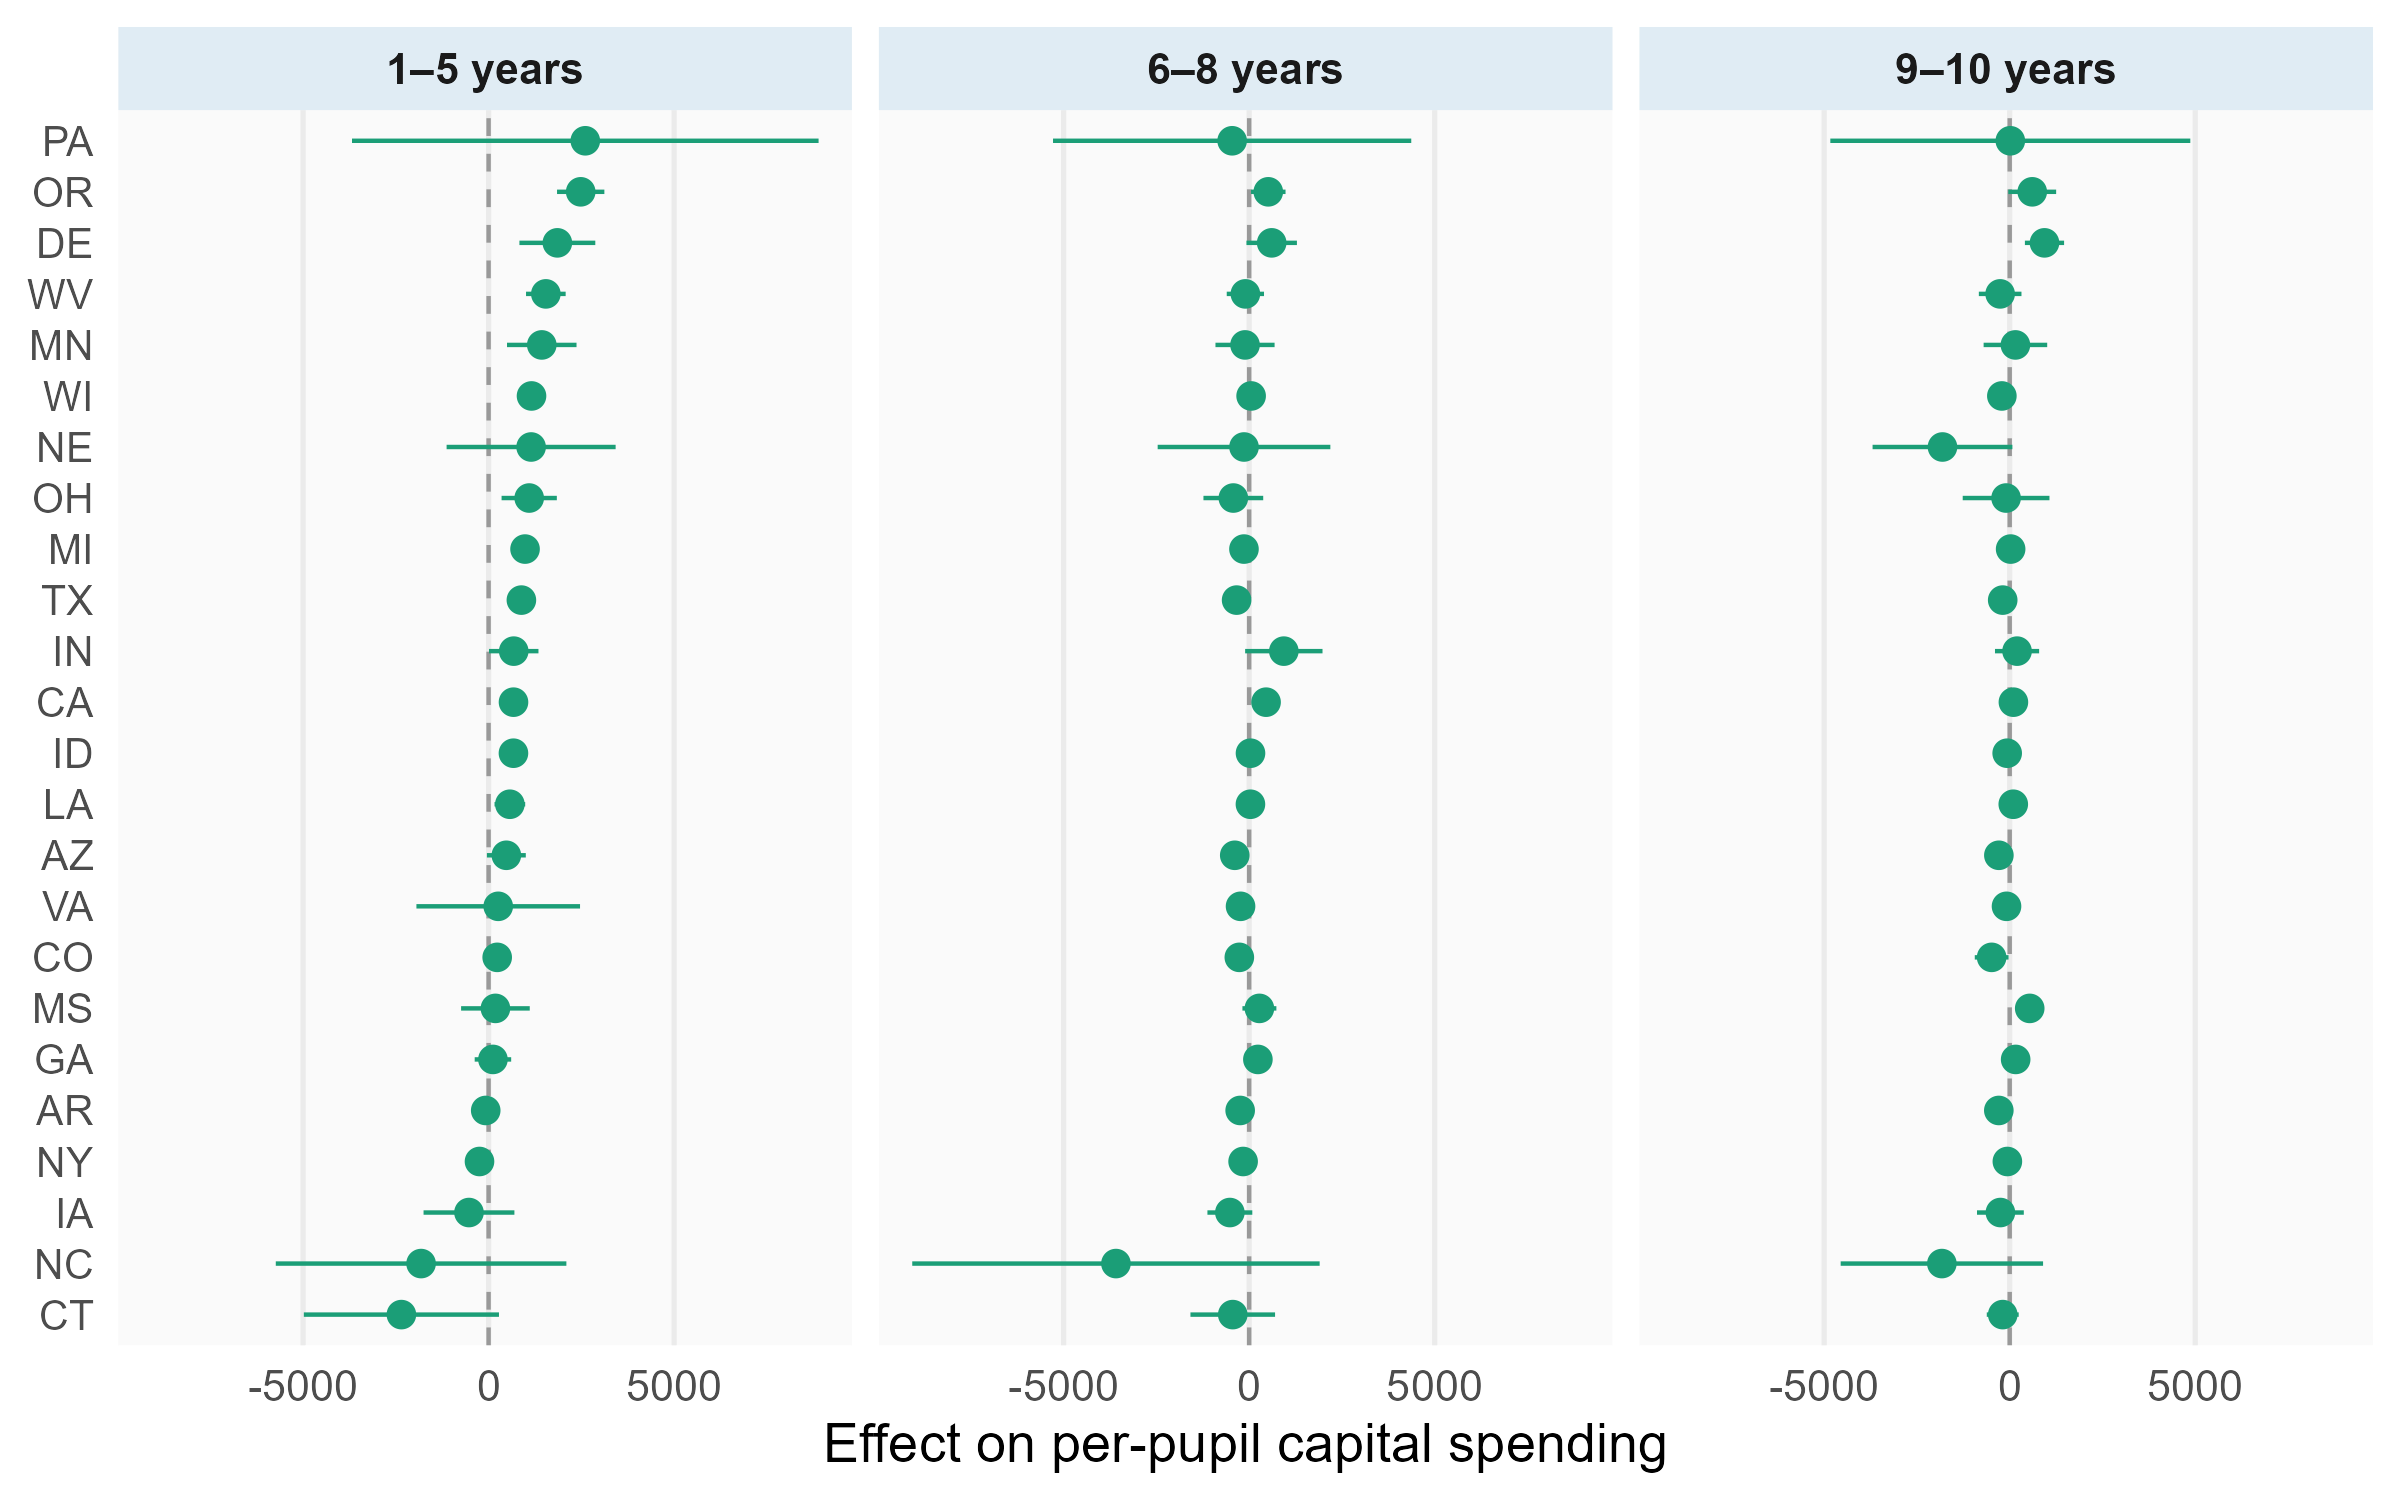
\includegraphics[width=0.99\textwidth]{images/forest_capital.png}
    \caption{Effect of School Levy on Capital Expenditures per Pupil by State}
    \label{fig:capital_forest}
\end{figure}

By the medium term (years 6--8), many states experience a decline in capital spending relative to the initial surge, consistent with the completion of major construction projects. Arizona, Arkansas, Colorado, Iowa, and Texas show significant negative coefficients in this window, indicating that capital expenditures fall below pre-election levels. Interestingly, some states maintain elevated spending: California (\$456), Oregon (\$515), and Delaware (\$607) continue to exhibit positive effects, suggesting either more gradual implementation or sustained investment in ongoing facility improvements. The long-run effects (years 9--10) are generally smaller in magnitude and often statistically insignificant, although Delaware and Mississippi stand out with persistent positive impacts, while Arizona, Arkansas, Colorado, Iowa, Nebraska, and Wisconsin show significant declines.



\subsection{Reduced-Form Effects on Test Scores}

The variation in test score effects by states is shown in Figure \ref{fig:tests_forest} and Table \ref{tab:state_test_scores}. While \citet{biasi_what_2025} find positive average effects nationally, our state-level decomposition reveals that this aggregate pattern conceals substantial heterogeneity, including both large positive and large negative estimates. In the short run (years 1--4), only Delaware (0.295 SD) and Louisiana (0.268 SD) exhibit statistically significant positive effects. Interestingly, several states display negative short-run effects: Indiana (-0.213 SD), Virginia (-0.531 SD), Colorado (-0.120 SD), and West Virginia (-0.938 SD), although most estimates are imprecise. The medium-term effects (years 5--8) show similarly mixed patterns. Arkansas (0.050 SD), California (0.058 SD), Ohio (0.111 SD), and Iowa (0.518 SD) exhibit positive and significant impacts, with Iowa's estimate being particularly large. North Carolina's effect remains positive and significant (0.978 SD). However, Idaho (-0.100 SD), Michigan (-0.083 SD), Mississippi (-0.243 SD), Pennsylvania (-0.590 SD), and Virginia (-0.348 SD) all show significant negative effects in this window. The negative estimates in Pennsylvania and Virginia are especially noteworthy given their magnitude. By the long run (years 9--12), Arkansas (0.080 SD), California (0.054 SD), Colorado (0.120 SD), Ohio (0.178 SD), and Texas (0.075 SD) display modest but statistically significant positive effects, while Pennsylvania (-0.687 SD), Virginia (-0.205 SD), West Virginia (-1.721 SD), and Iowa (-0.284 SD) show persistent negative impacts.

\begin{figure}[htbp]
    \centering
    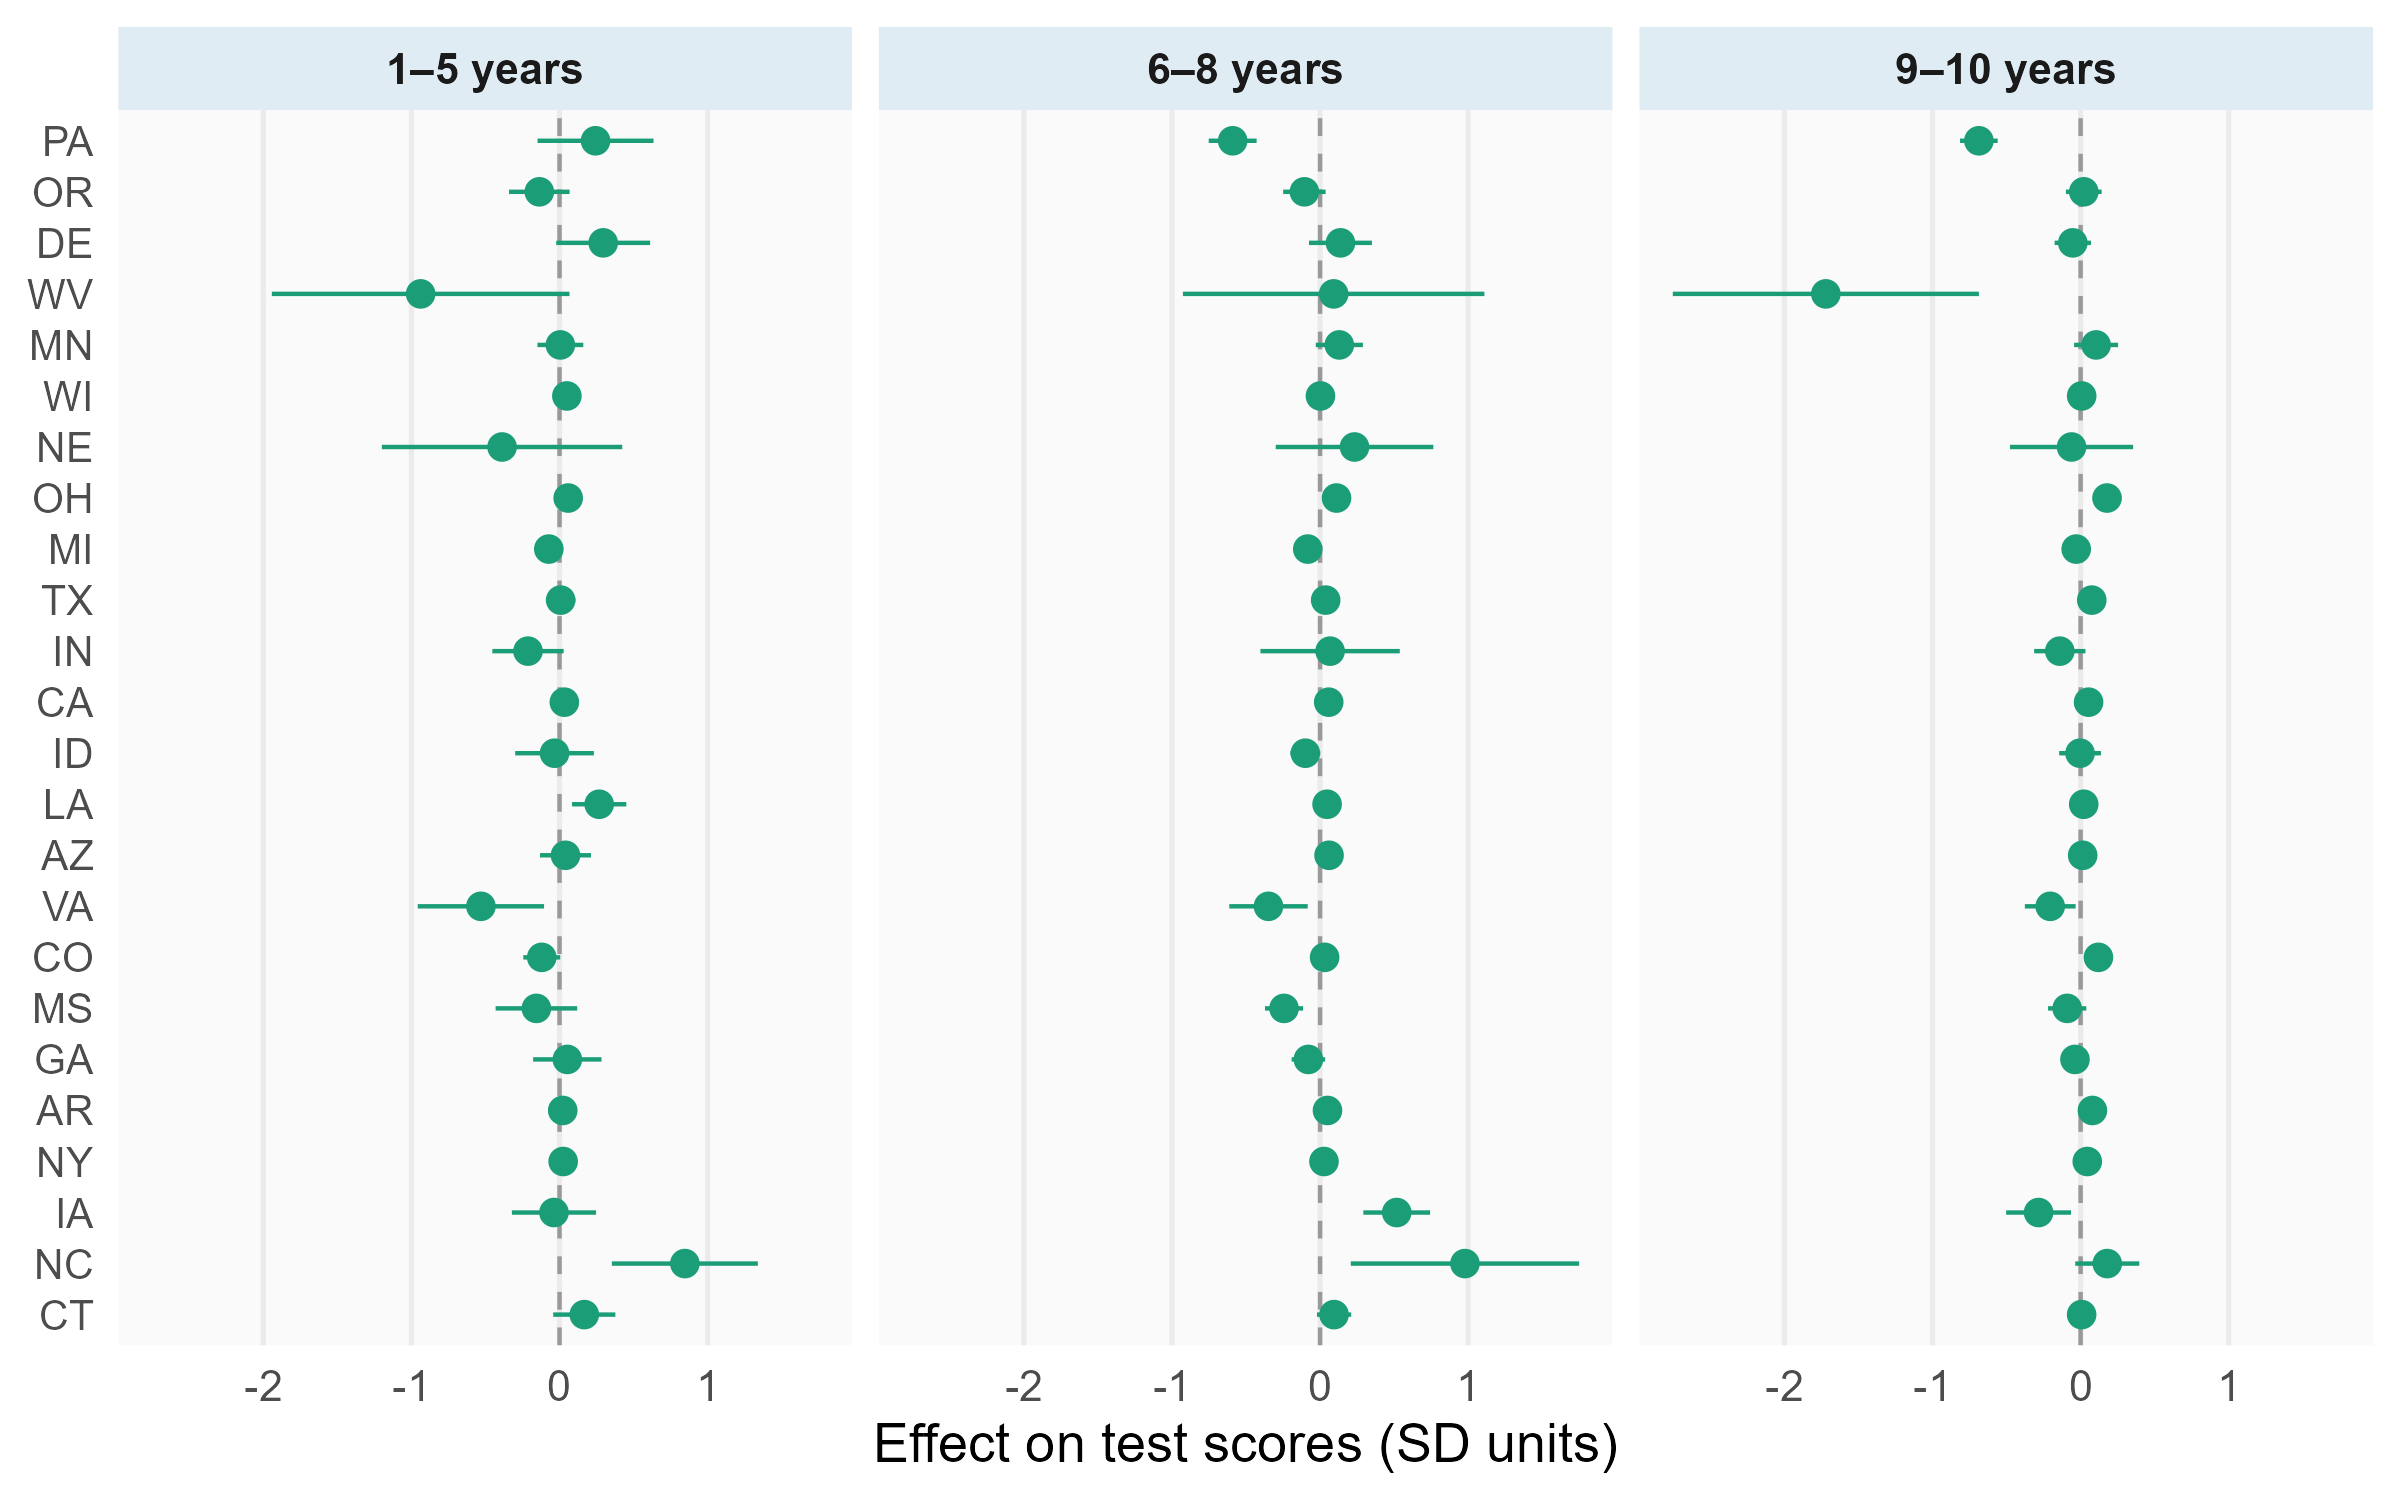
\includegraphics[width=0.99\textwidth]{images/forest_tests.png}
    \caption{Effect of School Levy on Test Scores by State}
    \label{fig:tests_forest}
\end{figure}

This heterogeneity raises important questions about the mechanisms underlying the national average effects. States with negative test score responses may differ in the types of projects funded, the quality of implementation, or the extent to which construction disrupts instruction. Alternatively, these patterns could reflect pre-existing differences in school infrastructure quality: states with relatively better facilities may see smaller gains or even declines if resources are diverted from instruction, while states with deteriorating infrastructure may benefit more from capital improvements.

\subsection{Housing Market Responses}

Figure \ref{fig:hpi_forest} and Table \ref{tab:state_house_prices} show that house price effects are similarly heterogeneous. In the short run (years 1--4), Louisiana exhibits a large positive effect (20.90 points on the HPI), while Virginia shows a marginally significant increase of 37.84 points. However, Idaho displays a substantial and significant \emph{negative} effect (-22.81 points), and Arkansas shows a smaller negative coefficient (-3.12 points). Most other states exhibit statistically insignificant short-run price responses, suggesting that housing markets may not immediately capitalize the benefits of school capital investments in all contexts.

The medium-term effects (years 5--8) reveal continued divergence. Louisiana (7.88 points), Minnesota (10.61 points), and Mississippi (10.00 points) show positive and significant house price increases, indicating that markets in these states eventually recognize and capitalize the improvements in school quality. In stark contrast, Connecticut (-5.23 points), Idaho (-20.92 points), Michigan (-6.54 points), and North Carolina (-44.78 points) exhibit significant negative effects, with North Carolina's estimate being especially large. The negative house price effects could reflect several mechanisms: migration responses, tax capitalization if property taxes rise to service the bonds, or signaling effects if bond passage reveals negative information about district finances or infrastructure conditions.

\begin{figure}[htbp]
    \centering
    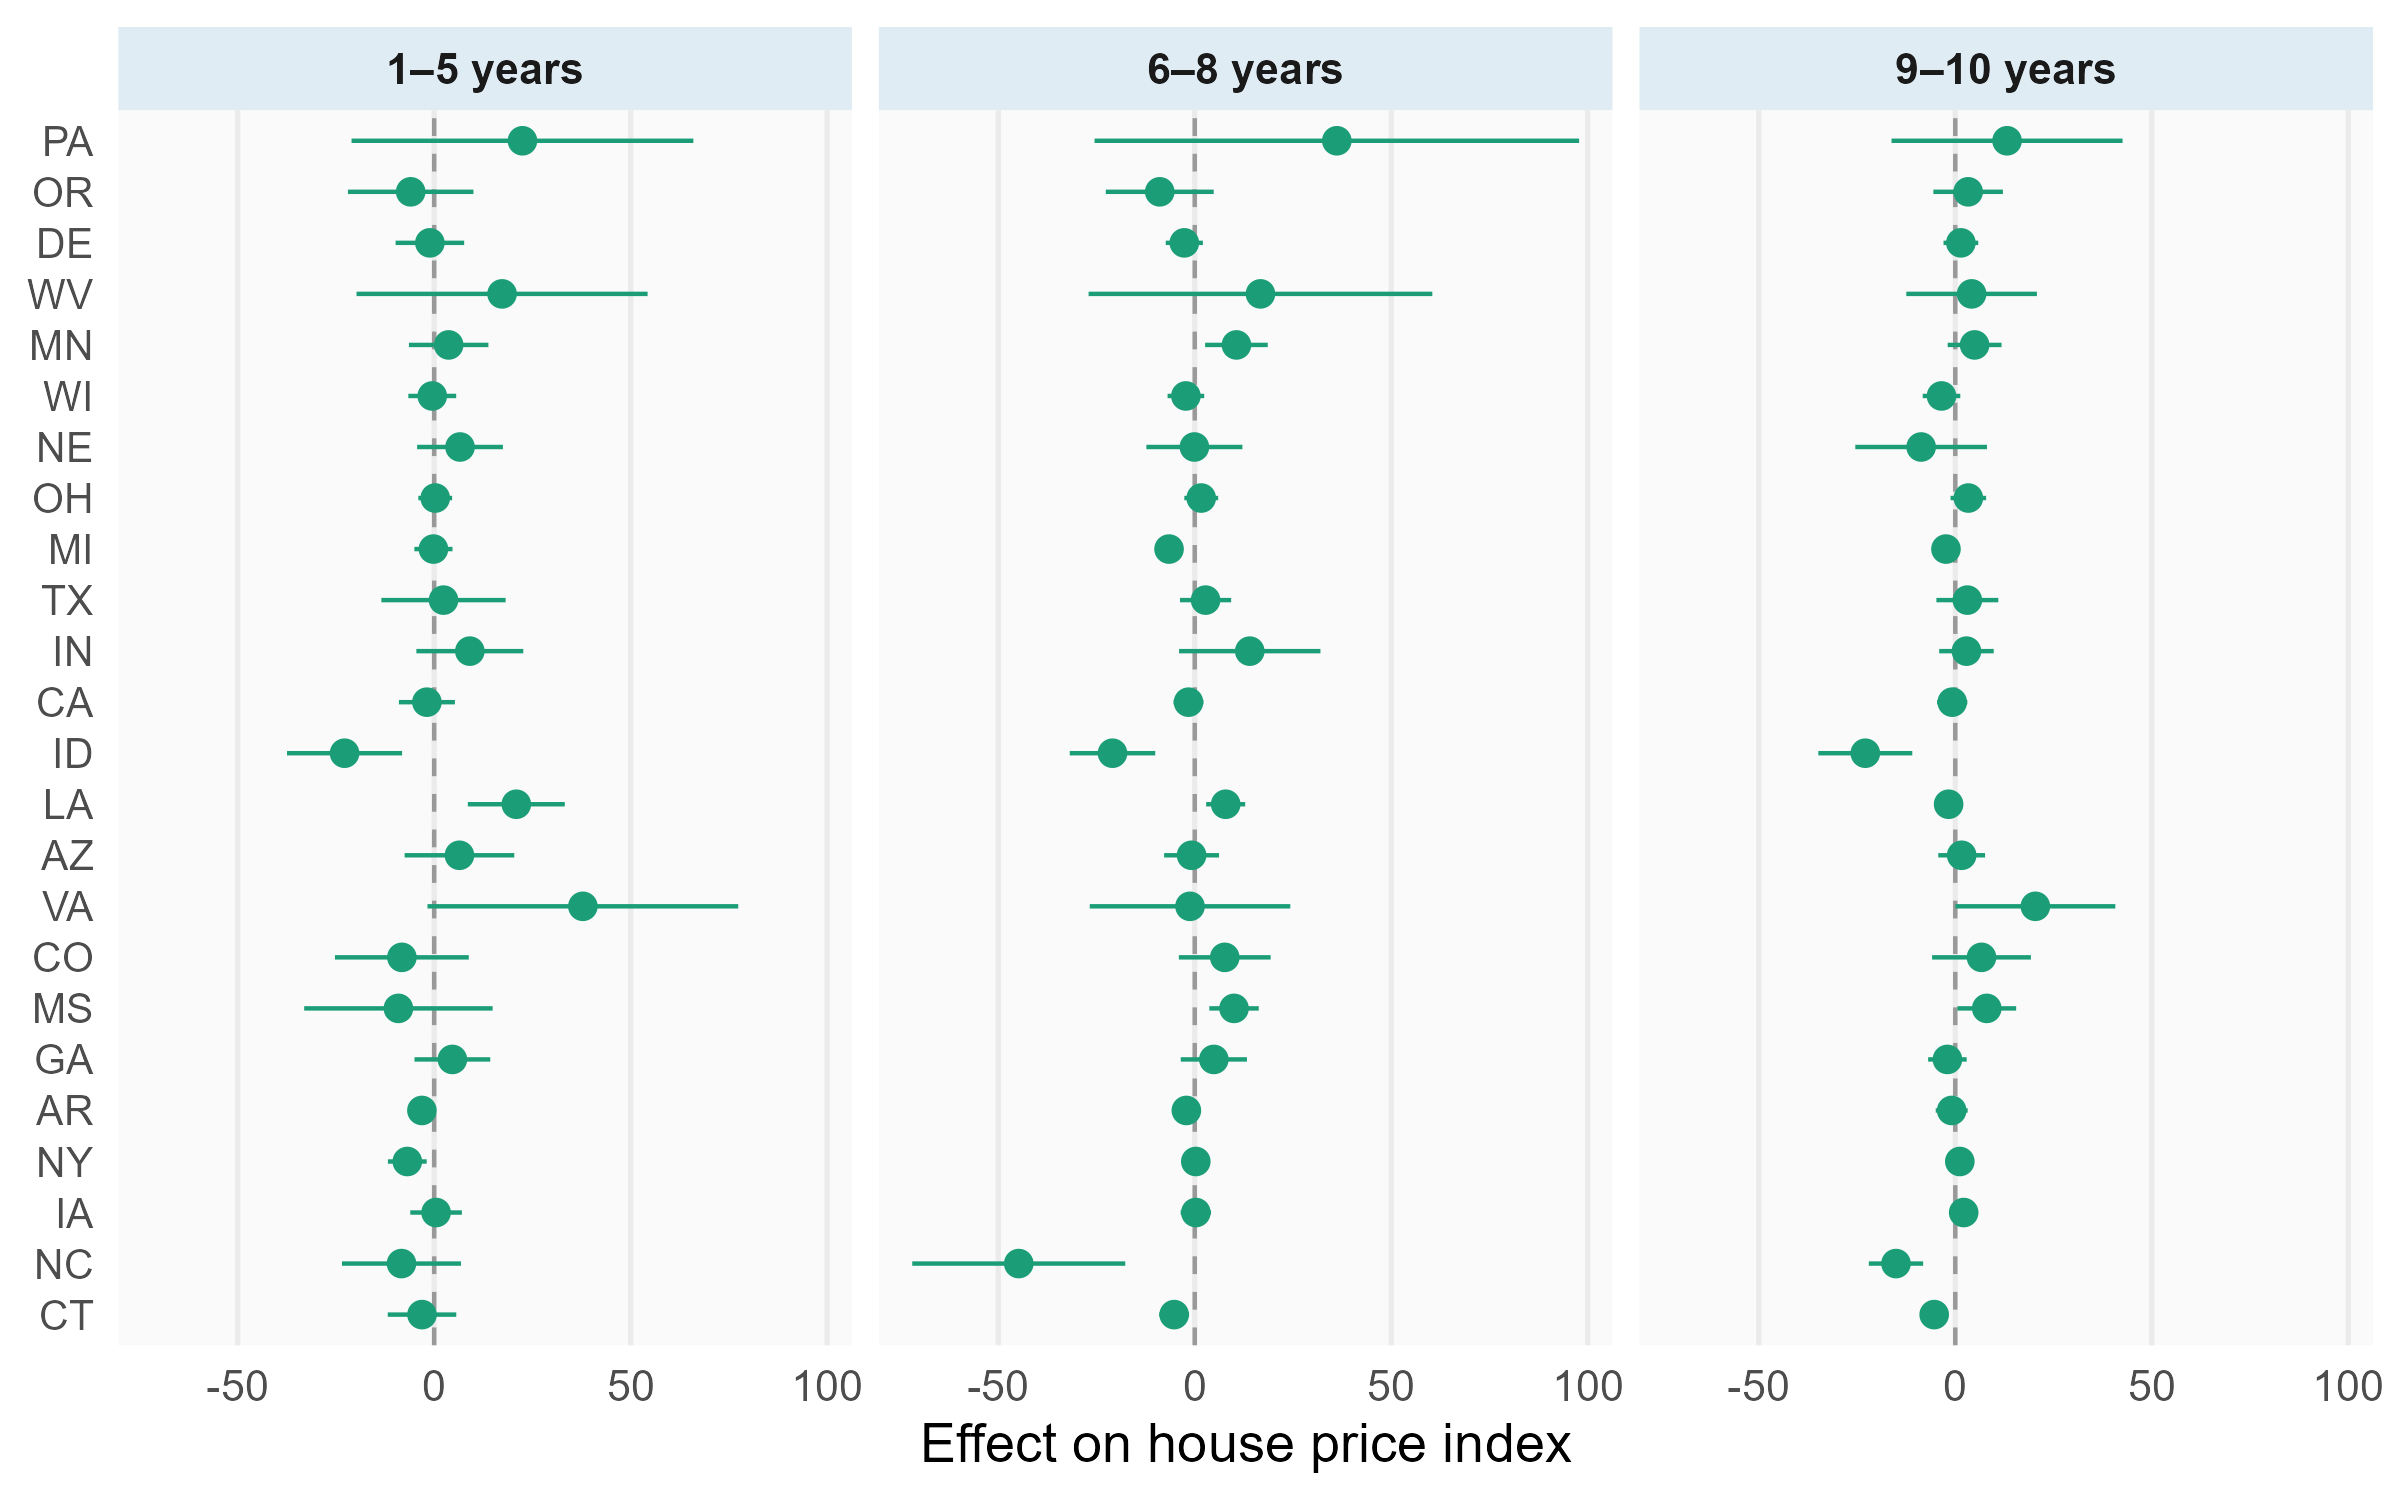
\includegraphics[width=0.99\textwidth]{images/forest_hpi.png}
    \caption{Effect of School Levy on Housing Price Index by State}
    \label{fig:hpi_forest}
\end{figure}

By the long run (years 9--12), house price effects are generally smaller and less precisely estimated. Connecticut (-5.37 points), Idaho (-22.90 points), and North Carolina (-15.09 points) maintain significant negative effects, while Iowa (2.14 points), Mississippi (8.01 points), and Virginia (20.38 points) show positive impacts. The persistence of negative effects in some states suggests that the housing market response is not merely a short-term adjustment but reflects sustained changes in neighborhood desirability or fiscal conditions.



